\documentclass[11pt,a4paper]{article}
\usepackage[top=2cm, bottom=2.3cm, left=1.8cm, right=1.8cm, headsep=0.8cm]{geometry}
\usepackage{amsmath,amssymb,amsfonts}
\usepackage{enumitem}
\usepackage{fancyhdr}
\usepackage[table]{xcolor}
\usepackage{tcolorbox}
\tcbuselibrary{breakable,skins}
\usepackage{tabularx}
\usepackage{multicol}
\usepackage{tikz}
\usetikzlibrary{arrows.meta,patterns,calc}

% High-Contrast Modern Color Palette
\definecolor{primaryDark}{RGB}{12, 32, 84}       % Midnight Navy (Deep)
\definecolor{primaryBlue}{RGB}{18, 72, 160}      % Solid Royal Blue
\definecolor{goldAccent}{RGB}{255, 215, 0}       % Gold highlight
\definecolor{l1Green}{RGB}{14, 120, 62}          % Vivid Forest Green (Level 1)
\definecolor{l2Amber}{RGB}{205, 80, 0}           % Rich Amber / Orange (Level 2)
\definecolor{l3Crimson}{RGB}{180, 20, 20}        % Deep Crimson Red (Level 3)
\definecolor{formulaBg}{RGB}{255, 252, 235}      % Warm Cream-Gold (Formula Callout)
\definecolor{formulaBorder}{RGB}{220, 160, 30}   % Gold Border for Formulas
\definecolor{cardBg}{RGB}{250, 252, 255}         % Clean Crisp Card Background
\definecolor{cardBorder}{RGB}{130, 170, 220}     % Sharp Steel Blue Border
\definecolor{tableStripe}{RGB}{242, 246, 252}    % Alternating Table Row
\definecolor{tableDarkHeader}{RGB}{12, 32, 84}   % Dark Table Header
\definecolor{darkCharcoal}{RGB}{25, 25, 25}      % High-contrast body text

% Page styling (Guaranteed Collision-Free Header)
\pagestyle{fancy}
\fancyhf{}
\setlength{\headheight}{16pt}
\fancyhead[L]{\small\textsf{\textbf{\textcolor{primaryDark}{StudyFAM JEE Revision}} $\vert$ \textbf{\textcolor{primaryBlue}{Day 01: Units, Measurements \& 1D Motion}}}}
\fancyhead[R]{\small\textsf{\textbf{\textcolor{l3Crimson}{Study Target: 8 Hours}}}}
\fancyfoot[C]{\textbf{\textsf{\thepage}}}
\renewcommand{\headrulewidth}{0.8pt}
\renewcommand{\footrulewidth}{0.4pt}

% Custom High-Contrast tcolorboxes
\tcbset{
  dayheader/.style={
    colback=primaryDark,
    coltext=white,
    boxrule=0pt,
    arc=3mm,
    left=14pt, right=14pt, top=10pt, bottom=10pt
  },
  sectionbanner/.style={
    colback=primaryBlue,
    coltext=white,
    boxrule=0pt,
    arc=2mm,
    left=10pt, right=10pt, top=6pt, bottom=6pt
  },
  chapterbanner/.style={
    colback=primaryDark,
    coltext=white,
    boxrule=0pt,
    arc=2mm,
    left=10pt, right=10pt, top=7pt, bottom=7pt
  },
  l1banner/.style={
    colback=l1Green,
    coltext=white,
    boxrule=0pt,
    arc=2mm,
    left=10pt, right=10pt, top=6pt, bottom=6pt
  },
  l2banner/.style={
    colback=l2Amber,
    coltext=white,
    boxrule=0pt,
    arc=2mm,
    left=10pt, right=10pt, top=6pt, bottom=6pt
  },
  l3banner/.style={
    colback=l3Crimson,
    coltext=white,
    boxrule=0pt,
    arc=2mm,
    left=10pt, right=10pt, top=6pt, bottom=6pt
  },
  formulacard/.style={
    enhanced,
    breakable,
    colback=formulaBg,
    colframe=formulaBorder,
    boxrule=1.2pt,
    arc=2mm,
    left=10pt, right=10pt, top=8pt, bottom=8pt
  },
  theorycard/.style={
    enhanced,
    breakable,
    colback=cardBg,
    colframe=cardBorder,
    boxrule=1.2pt,
    arc=2.5mm,
    left=12pt, right=12pt, top=10pt, bottom=10pt
  }
}

\begin{document}

% ==================== DAY HEADER BANNER ====================
\begin{tcolorbox}[dayheader]
\begin{center}
  {\Large \textbf{\textsf{\textcolor{goldAccent}{STUDYFAM JEE INTENSIVE REVISION SERIES}}}}\\[3pt]
  {\LARGE \textbf{\textsf{DAY 01: UNITS, MEASUREMENTS \& MOTION IN 1D}}}\\[5pt]
  {\normalsize \textbf{\textsf{Core Topics:}} Units \& Dimensions $\vert$ Error Propagation $\vert$ 1D Kinematics $\vert$ Graphs $\vert$ Relative Motion}\\[3pt]
  {\footnotesize \textbf{Daily Target Time:} 8 Hours \quad $\vert$ \quad \textbf{Curated Questions:} 75 Questions (25 Level-1 + 25 Level-2 + 25 Level-3)}
\end{center}
\end{tcolorbox}

\vspace{6pt}

% ==================== PART 1: TODAY'S PLAN ====================
\begin{tcolorbox}[sectionbanner]
  {\large \textbf{\textsf{PART 1: TODAY'S 8-HOUR ACTION SCHEDULE}}}
\end{tcolorbox}
\vspace{2pt}

\begin{center}
\renewcommand{\arraystretch}{1.25}
\small
\begin{tabularx}{\textwidth}{|c|c|X|c|}
\hline
\rowcolor{tableDarkHeader}
\textcolor{white}{\textbf{Session}} & \textcolor{white}{\textbf{Time}} & \textcolor{white}{\textbf{Focus Area \& High-Yield Strategy}} & \textcolor{white}{\textbf{Duration}} \\
\hline
\rowcolor{white}
\textbf{Block 1} & 09:00 -- 11:00 & \textbf{Theory \& Formula Compendium:} Study the unabridged theory section below. Review base units, dimensional formulas, error propagation rules, and 1D kinematic derivations. & 2.0 Hours \\
\hline
\rowcolor{tableStripe}
\textbf{Block 2} & 11:15 -- 12:45 & \textbf{Level-1 Foundation \& Speed Drill (Q1--Q25):} Direct formula application, dimensional checks, significant figures. Target: $\le 1.5$ min/Q. & 1.5 Hours \\
\hline
\rowcolor{white}
-- & 12:45 -- 01:45 & \textit{Lunch Break, Physical Movement \& Mental Recovery} & 1.0 Hour \\
\hline
\rowcolor{tableStripe}
\textbf{Block 3} & 01:45 -- 04:15 & \textbf{Level-2 Core JEE Main Mastery (Q26--Q50):} Moderate complexity, fractional errors, graphs ($x-t, v-t, a-t$), multi-body vertical motion. Target: $\le 2.5$ min/Q. & 2.5 Hours \\
\hline
\rowcolor{white}
\textbf{Block 4} & 04:30 -- 06:15 & \textbf{Level-3 Advanced \& Numerical Challenge (Q51--Q75):} Multi-concept calculus, variable acceleration, relative motion, integer numericals. & 1.75 Hours \\
\hline
\rowcolor{tableStripe}
\textbf{Block 5} & 06:30 -- 07:15 & \textbf{Master Answer Key Audit \& Error Logging:} Check answers, re-derive any missed questions, log tricky traps in your revision notebook. & 0.75 Hour \\
\hline
\rowcolor{tableDarkHeader}
\multicolumn{3}{|r|}{\textcolor{white}{\textbf{TOTAL DEDICATED STUDY TIME}}} & \textcolor{white}{\textbf{8.0 Hours}} \\
\hline
\end{tabularx}
\end{center}

\vspace{5pt}

% ==================== PART 2: OUTCOMES OF THE PLAN ====================
\begin{tcolorbox}[sectionbanner]
  {\large \textbf{\textsf{PART 2: TARGETED LEARNING OUTCOMES}}}
\end{tcolorbox}
\vspace{3pt}

\begin{itemize}[leftmargin=18pt,itemsep=2.5pt,topsep=1pt]
  \item[$\square$] \textbf{\textcolor{primaryDark}{Outcome 1 (Dimensions \& Homogeneity):}} Write dimensional formulas for mechanical/thermal constants ($G, h, \eta, k_B$) and find dimensions of unknown parameters using $[LHS] = [RHS]$.
  \item[$\square$] \textbf{\textcolor{primaryDark}{Outcome 2 (Error Analysis \& Propagation):}} Compute fractional and percentage errors in arbitrary power formulas $Z = A^p B^q / C^r$ using $\frac{\Delta Z}{Z} = p\frac{\Delta A}{A} + q\frac{\Delta B}{B} + r\frac{\Delta C}{C}$.
  \item[$\square$] \textbf{\textcolor{primaryDark}{Outcome 3 (Significant Figures \& Rounding):}} Apply Rules I, II, and III for rounding off numbers, especially the odd/even rule when the dropped digit is 5.
  \item[$\square$] \textbf{\textcolor{primaryDark}{Outcome 4 (Calculus Kinematics):}} Fluently transform between $x(t)$, $v(t)$, and $a(t)$ using $v = \frac{dx}{dt}$, $a = \frac{dv}{dt} = v\frac{dv}{dx}$, and definite integrals.
  \item[$\square$] \textbf{\textcolor{primaryDark}{Outcome 5 (Graphical Conversions):}} Rapidly determine velocity from slope of $x-t$, acceleration from slope of $v-t$, displacement from area under $v-t$, and velocity change from area under $a-t$.
  \item[$\square$] \textbf{\textcolor{primaryDark}{Outcome 6 (Gravity \& Galileo's Odd Numbers):}} Solve free fall and vertical projection problems instantly using $H = \frac{u^2}{2g}$, $T = \frac{2u}{g}$, $s_1:s_2:s_3 = 1:3:5$, and $h = \frac{1}{2}gt_1 t_2$.
  \item[$\square$] \textbf{\textcolor{primaryDark}{Outcome 7 (Relative Motion in 1D):}} Eliminate frame confusion in chasing, overtaking, and meeting problems using $\vec{v}_{A/B} = \vec{v}_A - \vec{v}_B$.
\end{itemize}

\vspace{5pt}

% ==================== PART 3: COMPLETE UNABRIDGED THEORY COMPENDIUM ====================
\begin{tcolorbox}[sectionbanner]
  {\large \textbf{\textsf{PART 3: UNABRIDGED THEORY \& FORMULA REVISION (FROM NOTES)}}}
\end{tcolorbox}
\vspace{4pt}

% -------------------------------------------------------------
% SUBSECTION 1: UNITS AND MEASUREMENTS
% -------------------------------------------------------------
\begin{tcolorbox}[chapterbanner]
  {\Large \textbf{\textsf{1. Units and Measurements (Complete Notes)}}}
\end{tcolorbox}
\vspace{4pt}

\noindent{\large\textbf{\textsf{\textcolor{primaryDark}{1.1 Fundamental vs. Derived Quantities}}}}\\[3pt]
\begin{itemize}[leftmargin=14pt,itemsep=2pt]
  \item \textbf{Fundamental (Base) Quantities:} Physical quantities that do not depend on any other physical quantities for their measurement.
  \begin{itemize}[leftmargin=12pt,itemsep=1pt]
    \item Mass ($\text{kg}$), Length ($\text{m}$), Time ($\text{s}$), Temperature ($\text{K}$), Electric Current ($\text{A}$), Luminous Intensity ($\text{cd}$), Amount of Substance ($\text{mol}$).
    \item \textit{Supplementary Quantities:} Plane angle ($\text{radian, rad}$), Solid angle ($\text{steradian, sr}$). Both are \textbf{dimensionless} ($[M^0 L^0 T^0]$) but possess units!
  \end{itemize}
  \item \textbf{Derived Quantities:} Physical quantities that can be expressed in terms of fundamental quantities (e.g., Velocity $[LT^{-1}]$, Acceleration $[LT^{-2}]$, Force $[MLT^{-2}]$, Work/Energy $[ML^2T^{-2}]$).
\end{itemize}

\vspace{5pt}
\noindent{\large\textbf{\textsf{\textcolor{primaryDark}{1.2 Systems of Units}}}}\\[3pt]
\begin{itemize}[leftmargin=14pt,itemsep=1pt]
  \item \textbf{FPS System:} Length in foot ($\text{ft}$), Mass in pound ($\text{lb}$), Time in second ($\text{s}$).
  \item \textbf{CGS System:} Length in centimetre ($\text{cm}$), Mass in gram ($\text{g}$), Time in second ($\text{s}$).
  \item \textbf{MKS System:} Length in metre ($\text{m}$), Mass in kilogram ($\text{kg}$), Time in second ($\text{s}$).
  \item \textbf{SI System (International System):} Modern extended MKS system covering 7 fundamental and 2 supplementary units.
\end{itemize}

\vspace{5pt}
\noindent{\large\textbf{\textsf{\textcolor{primaryDark}{1.3 Dimensions \& Dimensional Formulas}}}}\\[3pt]
The fundamental or base quantities along with the powers to which they are raised to express a physical quantity are called \textbf{dimensions}.
\begin{center}
\renewcommand{\arraystretch}{1.25}
\small
\begin{tabularx}{\linewidth}{|>{\raggedright\arraybackslash}X|>{\centering\arraybackslash}m{2.4cm}||>{\raggedright\arraybackslash}X|>{\centering\arraybackslash}m{2.8cm}|}
\hline
\rowcolor{tableDarkHeader}
\textcolor{white}{\textbf{Physical Quantity}} & \textcolor{white}{\textbf{Dimensions}} & \textcolor{white}{\textbf{Physical Quantity}} & \textcolor{white}{\textbf{Dimensions}} \\
\hline
\rowcolor{white}
Velocity / Speed & $[M^0 L T^{-1}]$ & Pressure / Stress / Modulus & $[M L^{-1} T^{-2}]$ \\
\hline
\rowcolor{tableStripe}
Acceleration & $[M^0 L T^{-2}]$ & Surface Tension / Spring Const. & $[M L^0 T^{-2}]$ \\
\hline
\rowcolor{white}
Force / Weight & $[M L T^{-2}]$ & Viscosity Coefficient ($\eta$) & $[M L^{-1} T^{-1}]$ \\
\hline
\rowcolor{tableStripe}
Work / Energy / Torque & $[M L^2 T^{-2}]$ & Gravitational Constant ($G$) & $[M^{-1} L^3 T^{-2}]$ \\
\hline
\rowcolor{white}
Power & $[M L^2 T^{-3}]$ & Planck's Const. ($h$) / Ang. Mom. & $[M L^2 T^{-1}]$ \\
\hline
\rowcolor{tableStripe}
Linear Momentum / Impulse & $[M L T^{-1}]$ & Boltzmann Constant ($k_B$) & $[M L^2 T^{-2} K^{-1}]$ \\
\hline
\end{tabularx}
\end{center}

\vspace{4pt}
\noindent{\large\textbf{\textsf{\textcolor{primaryDark}{1.4 Principle of Homogeneity of Dimensions}}}}\\[3pt]
According to this principle, the physical quantities having the same dimensions can be added or subtracted with each other, and in any physically valid equation, the dimensions of all terms on both sides must be identical:
\[
  \text{For example, in the equation } F = \frac{B}{A} m + \frac{C}{v}, \quad [F] = \left[\frac{B}{A}m\right] = \left[\frac{C}{v}\right]
\]

\begin{tcolorbox}[formulacard]
  \textbf{\textcolor{l3Crimson}{Crucial Rule for Non-Algebraic Functions:}}
  The arguments of trigonometric, exponential, and logarithmic functions are strictly \textbf{dimensionless}:
  \[
    \text{In } y = A \sin(\omega t - kx + \phi) \implies [\omega t] = [kx] = [\phi] = [M^0 L^0 T^0] = 1 \implies [\omega] = [T^{-1}], \ [k] = [L^{-1}].
  \]
  \[
    \text{In } P = P_0 e^{-\alpha t / \beta} \implies \left[\frac{\alpha t}{\beta}\right] = 1.
  \]
\end{tcolorbox}

\vspace{4pt}
\noindent{\large\textbf{\textsf{\textcolor{primaryDark}{1.5 Applications \& Limitations of Dimensional Analysis}}}}\\[3pt]
\begin{itemize}[leftmargin=14pt,itemsep=1pt]
  \item \textbf{Applications:}
    \begin{enumerate}[label=(\roman*),itemsep=1pt]
      \item To check the correctness of a given physical equation.
      \item To establish relations between physical quantities dimensionally (e.g., $T = 2\pi\sqrt{l/g}$).
      \item To convert the value of a physical quantity from one system of units to another ($n_1 u_1 = n_2 u_2$).
    \end{enumerate}
  \item \textbf{Limitations (From Notes):}
    \begin{enumerate}[label=(\roman*),itemsep=1pt]
      \item It does not predict the numerical dimensionless constant (e.g., the factor of $2\pi$ or $1/2$).
      \item It fails if a quantity depends on trigonometric, exponential, or logarithmic functions.
      \item It fails to derive a relationship if a physical quantity depends on more than three base variables (in mechanics).
      \item It cannot determine whether a quantity is a scalar or a vector.
    \end{enumerate}
\end{itemize}

\vspace{5pt}
\noindent{\large\textbf{\textsf{\textcolor{primaryDark}{1.6 Rules for Rounding Off Numbers (From Notes)}}}}\\[3pt]
\begin{itemize}[leftmargin=14pt,itemsep=1pt]
  \item \textbf{Rule I:} If the digit to be dropped is more than $5$, the preceding digit is increased by one (e.g., $6.87 \approx 6.9$).
  \item \textbf{Rule II:} If the digit to be dropped is less than $5$, the preceding digit is left unchanged (e.g., $3.94 \approx 3.9$).
  \item \textbf{Rule III:} If the digit to be dropped is exactly $5$:
    \begin{itemize}[leftmargin=12pt,itemsep=1pt]
      \item If the preceding digit is \textbf{odd}, it is increased by one (e.g., $14.35 \approx 14.4$).
      \item If the preceding digit is \textbf{even}, it is left unchanged (e.g., $14.45 \approx 14.4$).
    \end{itemize}
\end{itemize}

\vspace{5pt}
\noindent{\large\textbf{\textsf{\textcolor{primaryDark}{1.7 Rules for Significant Figures}}}}\\[3pt]
\begin{itemize}[leftmargin=14pt,itemsep=1pt]
  \item All non-zero digits are significant (e.g., $123.45$ has 5 significant figures).
  \item All zeros between two non-zero digits are significant (e.g., $23.023$ has 5 significant figures).
  \item Leading zeros (to the left of the first non-zero digit) are NEVER significant (e.g., $0.0003$ has 1 significant figure).
  \item Trailing zeros after a decimal point are significant (e.g., $2.10$ has 3 significant figures).
  \item Exponential powers of 10 do not affect significant figures (e.g., $2.1 \times 10^{-3}$ has 2 significant figures).
\end{itemize}

\vspace{5pt}
\noindent{\large\textbf{\textsf{\textcolor{primaryDark}{1.8 Representation of Errors \& Combination Rules (From Notes)}}}}\\[3pt]
\begin{itemize}[leftmargin=14pt,itemsep=1pt]
  \item \textbf{Mean Value:} $a_m = \dfrac{a_1 + a_2 + \dots + a_n}{n} = \dfrac{1}{n}\sum_{i=1}^n a_i$.
  \item \textbf{Absolute Error:} $\Delta a_i = |a_m - a_i|$.
  \item \textbf{Mean Absolute Error:} $\overline{\Delta a} = \dfrac{\Delta a_1 + \Delta a_2 + \dots + \Delta a_n}{n} = \dfrac{1}{n}\sum_{i=1}^n \Delta a_i$.
  \item \textbf{Final Reported Measurement:} $a = a_m \pm \overline{\Delta a}$.
  \item \textbf{Relative (Fractional) Error:} $\dfrac{\text{Mean Absolute Error}}{\text{Mean Value}} = \dfrac{\overline{\Delta a}}{a_m}$.
  \item \textbf{Percentage Error:} $\dfrac{\overline{\Delta a}}{a_m} \times 100\%$.
\end{itemize}

\begin{tcolorbox}[formulacard]
  \textbf{\textcolor{primaryDark}{Error Propagation Laws:}}
  \begin{itemize}[leftmargin=12pt,itemsep=2pt]
    \item \textbf{In Sum ($Z = A + B$):} $\Delta Z = \Delta A + \Delta B$; \quad Maximum fractional error: $\dfrac{\Delta Z}{Z} = \dfrac{\Delta A + \Delta B}{A + B}$.
    \item \textbf{In Difference ($Z = A - B$):} $\Delta Z = \Delta A + \Delta B$; \quad Maximum fractional error: $\dfrac{\Delta Z}{Z} = \dfrac{\Delta A + \Delta B}{A - B}$.
    \item \textbf{In Product ($Z = AB$):} $\dfrac{\Delta Z}{Z} = \dfrac{\Delta A}{A} + \dfrac{\Delta B}{B}$.
    \item \textbf{In Division ($Z = A / B$):} $\dfrac{\Delta Z}{Z} = \dfrac{\Delta A}{A} + \dfrac{\Delta B}{B}$.
    \item \textbf{In Powers ($Z = A^n$):} $\dfrac{\Delta Z}{Z} = n \dfrac{\Delta A}{A}$.
    \item \textbf{General Power Product Form:} If $Z = \dfrac{A^x B^y}{C^q}$, the maximum fractional error is:
    \[
      \frac{\Delta Z}{Z} = x\left(\frac{\Delta A}{A}\right) + y\left(\frac{\Delta B}{B}\right) + q\left(\frac{\Delta C}{C}\right)
    \]
  \end{itemize}
\end{tcolorbox}

\vspace{10pt}

% -------------------------------------------------------------
% SUBSECTION 2: MOTION IN A STRAIGHT LINE
% -------------------------------------------------------------
\begin{tcolorbox}[chapterbanner]
  {\Large \textbf{\textsf{2. Motion in a Straight Line (Complete Notes)}}}
\end{tcolorbox}
\vspace{4pt}

\noindent{\large\textbf{\textsf{\textcolor{primaryDark}{2.1 Distance versus Displacement}}}}\\[3pt]
\begin{itemize}[leftmargin=14pt,itemsep=1pt]
  \item \textbf{Distance:} Total length of path covered by the particle. It is a scalar, always positive for a moving particle, and never decreases with time.
  \item \textbf{Displacement:} Minimum straight-line distance directed from initial position to final position:
  \[
    \Delta \vec{r} = \vec{r}_B - \vec{r}_A = (x_2 - x_1)\hat{i} + (y_2 - y_1)\hat{j} + (z_2 - z_1)\hat{k}
  \]
\end{itemize}

\vspace{5pt}
\noindent{\large\textbf{\textsf{\textcolor{primaryDark}{2.2 Velocity and Acceleration Definitions}}}}\\[3pt]
\begin{itemize}[leftmargin=14pt,itemsep=1pt]
  \item \textbf{Average Velocity:} $\vec{v}_{\text{avg}} = \dfrac{\text{Displacement}}{\text{Time interval}} = \dfrac{\Delta \vec{r}}{\Delta t}$.
  \item \textbf{Average Speed:} $\text{Average Speed} = \dfrac{\text{Total Distance travelled}}{\text{Total Time interval}}$.
  \item \textbf{Instantaneous Velocity:} $\vec{v} = \dfrac{d\vec{r}}{dt} = \dfrac{dx}{dt}\hat{i} + \dfrac{dy}{dt}\hat{j} + \dfrac{dz}{dt}\hat{k} = v_x \hat{i} + v_y \hat{j} + v_z \hat{k}$.
  \item \textbf{Average Acceleration:} $\vec{a}_{\text{avg}} = \dfrac{\text{Total change in velocity}}{\text{Total time taken}} = \dfrac{\Delta \vec{v}}{\Delta t}$.
  \item \textbf{Instantaneous Acceleration:} $\vec{a} = \dfrac{d\vec{v}}{dt} = \dfrac{dv_x}{dt}\hat{i} + \dfrac{dv_y}{dt}\hat{j} + \dfrac{dv_z}{dt}\hat{k} = a_x \hat{i} + a_y \hat{j} + a_z \hat{k}$.
\end{itemize}

\vspace{5pt}
\noindent{\large\textbf{\textsf{\textcolor{primaryDark}{2.3 Fundamental Rules of 1D Motion}}}}\\[3pt]
\begin{itemize}[leftmargin=14pt,itemsep=1pt]
  \item $\text{Distance} \ge |\text{displacement}|$ and $\text{Average speed} \ge |\text{average velocity}|$.
  \item If $\text{Distance} > |\text{displacement}|$, the particle must have reversed its direction of motion at least once (instantaneous velocity $v = 0$ at the turning point).
  \item \textbf{Calculus Progression:}
  \[
    \text{Displacement } x \xrightarrow{\text{Differentiation } \frac{d}{dt}} \text{Velocity } v \xrightarrow{\text{Differentiation } \frac{d}{dt}} \text{Acceleration } a
  \]
  \[
    \text{Acceleration } a \xrightarrow{\text{Integration } \int dt} \text{Velocity } v \xrightarrow{\text{Integration } \int dt} \text{Displacement } x
  \]
  \item In 1D with space-dependence: $a = \dfrac{dv}{dt} = \dfrac{dv}{dx}\dfrac{dx}{dt} = v\dfrac{dv}{dx} \implies \int v\,dv = \int a\,dx$.
\end{itemize}

\vspace{5pt}
\noindent{\large\textbf{\textsf{\textcolor{primaryDark}{2.4 Equations of Motion (Constant Acceleration)}}}}\\[3pt]
\begin{itemize}[leftmargin=14pt,itemsep=1pt]
  \item \textbf{In Vector Form:}
  \[
    \vec{v} = \vec{u} + \vec{a}t, \quad \Delta \vec{r} = \left(\frac{\vec{u}+\vec{v}}{2}\right)t = \vec{u}t + \frac{1}{2}\vec{a}t^2 = \vec{v}t - \frac{1}{2}\vec{a}t^2, \quad v^2 = u^2 + 2\vec{a}\cdot\vec{s}, \quad \vec{s}_{n^{\text{th}}} = \vec{u} + \frac{\vec{a}}{2}(2n - 1)
  \]
  \item \textbf{In Scalar Form (1D Rectilinear):}
  \[
    v = u + at, \quad s = \left(\frac{u+v}{2}\right)t, \quad s = ut + \frac{1}{2}at^2, \quad s = vt - \frac{1}{2}at^2, \quad v^2 = u^2 + 2as, \quad s_n = u + \frac{a}{2}(2n - 1)
  \]
  \item \textbf{Uniform Motion:} If an object moving along a straight line covers equal distances in equal intervals of time, acceleration $a = 0$ and $s = vt$.
\end{itemize}

\begin{tcolorbox}[formulacard]
  \textbf{\textcolor{l3Crimson}{2.5 Motion Under Gravity (All 8 Specific Theorems From Notes)}}
  \textit{Taking upward direction as positive ($a = -g$):}
  \begin{enumerate}[label=(\roman*),leftmargin=14pt,itemsep=2pt]
    \item \textbf{Maximum Height Attained:} $H = \dfrac{u^2}{2g}$.
    \item \textbf{Time of Ascent \& Descent:} $t_{\text{ascent}} = t_{\text{descent}} = \dfrac{u}{g}$.
    \item \textbf{Total Time of Flight:} $T = \dfrac{2u}{g}$.
    \item \textbf{Final Speed at Projection Level:} Speed returning to starting level is equal to initial projection speed $u$ (directed downwards).
    \item \textbf{Galileo's Law of Odd Numbers:} For a body falling freely from rest, the ratio of successive distances covered in equal consecutive time intervals $t$ is:
    \[
      S_1 : S_2 : S_3 : \dots : S_n = 1 : 3 : 5 : 7 : \dots : (2n - 1)
    \]
    \item \textbf{Speed Symmetry:} At any horizontal level along its path, the body has identical speed during its upward and downward journeys.
    \item \textbf{Two-Time Crossing Rule:} If a body thrown vertically upwards crosses a given height $h$ at times $t_1$ and $t_2$:
    \[
      h = \frac{1}{2}g t_1 t_2, \quad t_1 + t_2 = \frac{2u}{g}, \quad H_{\max} = \frac{1}{8}g (t_1 + t_2)^2
    \]
    \item \textbf{Three-Body Projection Theorem:} If three bodies are projected from the top of a tower of height $H$ with the same initial speed $v$ (one vertically upward, one vertically downward, and one horizontally) taking times $t_1, t_2$, and $t_3$ respectively to reach the ground:
    \[
      t_3 = \sqrt{t_1 t_2} \quad \text{and} \quad H = \frac{1}{2}g t_1 t_2
    \]
  \end{enumerate}
\end{tcolorbox}

\vspace{5pt}
\noindent{\large\textbf{\textsf{\textcolor{primaryDark}{2.6 Complete Graph Masterclass (From Notes)}}}}\\[3pt]

\begin{center}
\resizebox{0.96\linewidth}{!}{
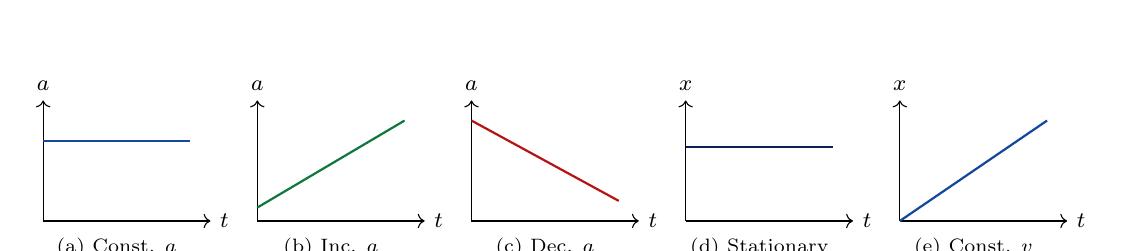
\begin{tikzpicture}[scale=0.85]
  % 1. a-t Constant
  \draw[->] (0,0) -- (2.5,0) node[right]{\footnotesize $t$};
  \draw[->] (0,0) -- (0,1.8) node[above]{\footnotesize $a$};
  \draw[thick, primaryBlue] (0,1.2) -- (2.2,1.2);
  \node at (1.1,-0.4) {\scriptsize (a) Const. $a$};
  
  % 2. a-t Increasing
  \begin{scope}[xshift=3.2cm]
  \draw[->] (0,0) -- (2.5,0) node[right]{\footnotesize $t$};
  \draw[->] (0,0) -- (0,1.8) node[above]{\footnotesize $a$};
  \draw[thick, l1Green] (0,0.2) -- (2.2,1.5);
  \node at (1.1,-0.4) {\scriptsize (b) Inc. $a$};
  \end{scope}

  % 3. a-t Decreasing
  \begin{scope}[xshift=6.4cm]
  \draw[->] (0,0) -- (2.5,0) node[right]{\footnotesize $t$};
  \draw[->] (0,0) -- (0,1.8) node[above]{\footnotesize $a$};
  \draw[thick, l3Crimson] (0,1.5) -- (2.2,0.3);
  \node at (1.1,-0.4) {\scriptsize (c) Dec. $a$};
  \end{scope}

  % 4. x-t Stationary
  \begin{scope}[xshift=9.6cm]
  \draw[->] (0,0) -- (2.5,0) node[right]{\footnotesize $t$};
  \draw[->] (0,0) -- (0,1.8) node[above]{\footnotesize $x$};
  \draw[thick, primaryDark] (0,1.1) -- (2.2,1.1);
  \node at (1.1,-0.4) {\scriptsize (d) Stationary};
  \end{scope}

  % 5. x-t Constant v
  \begin{scope}[xshift=12.8cm]
  \draw[->] (0,0) -- (2.5,0) node[right]{\footnotesize $t$};
  \draw[->] (0,0) -- (0,1.8) node[above]{\footnotesize $x$};
  \draw[thick, primaryBlue] (0,0) -- (2.2,1.5);
  \node at (1.1,-0.4) {\scriptsize (e) Const. $v$};
  \end{scope}
\end{tikzpicture}
}
\end{center}

\vspace{2pt}

\begin{center}
\resizebox{0.96\linewidth}{!}{
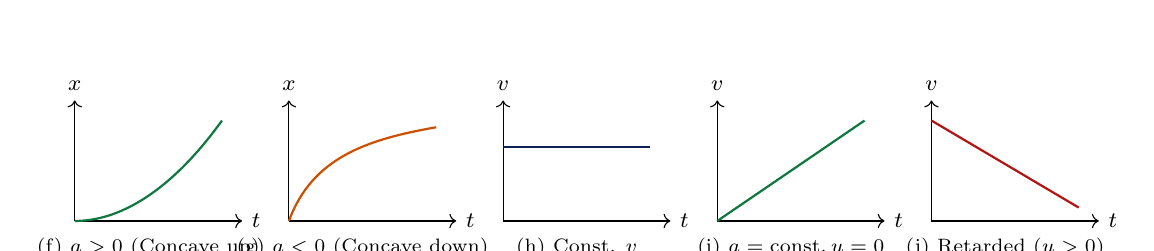
\begin{tikzpicture}[scale=0.85]
  % 6. x-t Accelerated
  \draw[->] (0,0) -- (2.5,0) node[right]{\footnotesize $t$};
  \draw[->] (0,0) -- (0,1.8) node[above]{\footnotesize $x$};
  \draw[thick, l1Green] (0,0) parabola (2.2,1.5);
  \node at (1.1,-0.4) {\scriptsize (f) $a > 0$ (Concave up)};

  % 7. x-t Retarded
  \begin{scope}[xshift=3.2cm]
  \draw[->] (0,0) -- (2.5,0) node[right]{\footnotesize $t$};
  \draw[->] (0,0) -- (0,1.8) node[above]{\footnotesize $x$};
  \draw[thick, l2Amber] (0,0) to[out=70,in=190] (2.2,1.4);
  \node at (1.1,-0.4) {\scriptsize (g) $a < 0$ (Concave down)};
  \end{scope}

  % 8. v-t Constant v
  \begin{scope}[xshift=6.4cm]
  \draw[->] (0,0) -- (2.5,0) node[right]{\footnotesize $t$};
  \draw[->] (0,0) -- (0,1.8) node[above]{\footnotesize $v$};
  \draw[thick, primaryDark] (0,1.1) -- (2.2,1.1);
  \node at (1.1,-0.4) {\scriptsize (h) Const. $v$};
  \end{scope}

  % 9. v-t Constant a (u=0)
  \begin{scope}[xshift=9.6cm]
  \draw[->] (0,0) -- (2.5,0) node[right]{\footnotesize $t$};
  \draw[->] (0,0) -- (0,1.8) node[above]{\footnotesize $v$};
  \draw[thick, l1Green] (0,0) -- (2.2,1.5);
  \node at (1.1,-0.4) {\scriptsize (i) $a = \text{const}, u=0$};
  \end{scope}

  % 10. v-t Retardation (u > 0)
  \begin{scope}[xshift=12.8cm]
  \draw[->] (0,0) -- (2.5,0) node[right]{\footnotesize $t$};
  \draw[->] (0,0) -- (0,1.8) node[above]{\footnotesize $v$};
  \draw[thick, l3Crimson] (0,1.5) -- (2.2,0.2);
  \node at (1.1,-0.4) {\scriptsize (j) Retarded ($u>0$)};
  \end{scope}
\end{tikzpicture}
}
\end{center}

\vspace{3pt}
\begin{itemize}[leftmargin=14pt,itemsep=1.5pt]
  \item \textbf{Slope of $x\text{--}t$ curve} $= \dfrac{dx}{dt} = \text{Velocity } v$.
  \item \textbf{Slope of $v\text{--}t$ curve} $= \dfrac{dv}{dt} = \text{Acceleration } a$.
  \item \textbf{Area under $v\text{--}t$ curve} $= \int v\,dt = \text{Displacement } \Delta x$.
  \item \textbf{Area under $a\text{--}t$ curve} $= \int a\,dt = \text{Change in Velocity } \Delta v$.
\end{itemize}

\newpage
\begin{tcolorbox}[l1banner]
  {\Large \textbf{\textsf{LEVEL 1: FOUNDATION \& SPEED DRILLS (25 Questions)}}}\\[2pt]
  {\footnotesize \textbf{Focus:} Direct Formula Application $\vert$ Dimensional Analysis $\vert$ Target Time: $\le 1.5$ min/Q}
\end{tcolorbox}
\vspace{6pt}

\begin{enumerate}[label=\textbf{\textcolor{l1Green}{Q\arabic*.}},leftmargin=24pt,itemsep=10pt]

  % Q1
  \item If $A$ and $B$ have different physical dimensions, then which of the following operations can be physically meaningful?
  \begin{multicols}{2}
  \begin{enumerate}[label=\textbf{\textcolor{primaryDark}{(\Alph*)}},itemsep=2pt]
    \item $A / B$
    \item $A - B$
    \item $A + B$
    \item $e^{A/B}$
  \end{enumerate}
  \end{multicols}

  % Q2
  \item If $x$ and $a$ represent distance, for what value of $n$ is the equation $\displaystyle\int \frac{dx}{\sqrt{a^2 - x^n}} = \sin^{-1}\left(\frac{x}{a}\right)$ dimensionally correct?
  \begin{multicols}{2}
  \begin{enumerate}[label=\textbf{\textcolor{primaryDark}{(\Alph*)}},itemsep=2pt]
    \item Zero
    \item $2$
    \item $-2$
    \item $1$
  \end{enumerate}
  \end{multicols}

  % Q3
  \item Young's modulus of a material has the same SI unit and dimensions as:
  \begin{multicols}{2}
  \begin{enumerate}[label=\textbf{\textcolor{primaryDark}{(\Alph*)}},itemsep=2pt]
    \item Pressure
    \item Energy
    \item Strain
    \item Force
  \end{enumerate}
  \end{multicols}

  % Q4
  \item Let $Q$ denote the charge on the plate of a capacitor of capacitance $C$. The dimensional formula of $\dfrac{Q^2}{C}$ is:
  \begin{multicols}{2}
  \begin{enumerate}[label=\textbf{\textcolor{primaryDark}{(\Alph*)}},itemsep=2pt]
    \item $[M L^2 T^{-2}]$
    \item $[M L T^{-2}]$
    \item $[M L^2 T^{-1}]$
    \item $[M^0 L^0 T^0]$
  \end{enumerate}
  \end{multicols}

  % Q5
  \item The dimensional representation of Planck's constant $h$ is identical to that of:
  \begin{multicols}{2}
  \begin{enumerate}[label=\textbf{\textcolor{primaryDark}{(\Alph*)}},itemsep=2pt]
    \item Linear momentum
    \item Energy
    \item Power
    \item Angular momentum
  \end{enumerate}
  \end{multicols}

  % Q6
  \item Of the following physical quantities, which one has dimensions different from the remaining three?
  \begin{multicols}{2}
  \begin{enumerate}[label=\textbf{\textcolor{primaryDark}{(\Alph*)}},itemsep=2pt]
    \item Work
    \item Torque
    \item Energy
    \item Angular momentum
  \end{enumerate}
  \end{multicols}

  % Q7
  \item The dimensional formula of shear modulus of rigidity $\eta$ is:
  \begin{multicols}{2}
  \begin{enumerate}[label=\textbf{\textcolor{primaryDark}{(\Alph*)}},itemsep=2pt]
    \item $[M L^{-1} T^{-2}]$
    \item $[M L T^{-2}]$
    \item $[M L^2 T^{-2}]$
    \item $[M L^{-2} T^{-1}]$
  \end{enumerate}
  \end{multicols}

  % Q8
  \item In an experiment, four quantities $a, b, c$, and $d$ are measured with percentage errors $1\%$, $2\%$, $3\%$, and $4\%$ respectively. A quantity $P$ is calculated as $P = \dfrac{a^3 b^2}{c d}$. The maximum percentage error in $P$ is:
  \begin{multicols}{2}
  \begin{enumerate}[label=\textbf{\textcolor{primaryDark}{(\Alph*)}},itemsep=2pt]
    \item $10\%$
    \item $7\%$
    \item $4\%$
    \item $14\%$
  \end{enumerate}
  \end{multicols}

  % Q9
  \item The percentage errors in measuring $M, L$, and $T$ are $1\%$, $1.5\%$, and $3\%$ respectively. Then the maximum percentage error in measuring the physical quantity with dimensions $[M L^{-1} T^{-1}]$ is:
  \begin{multicols}{2}
  \begin{enumerate}[label=\textbf{\textcolor{primaryDark}{(\Alph*)}},itemsep=2pt]
    \item $3.5\%$
    \item $7.5\%$
    \item $4.5\%$
    \item $5.5\%$
  \end{enumerate}
  \end{multicols}

  % Q10
  \item The respective number of significant figures for the numbers $23.023$, $0.0003$, and $2.1 \times 10^{-3}$ are:
  \begin{multicols}{2}
  \begin{enumerate}[label=\textbf{\textcolor{primaryDark}{(\Alph*)}},itemsep=2pt]
    \item $5, 1, 2$
    \item $5, 1, 5$
    \item $5, 5, 2$
    \item $4, 4, 2$
  \end{enumerate}
  \end{multicols}

  % Q11
  \item The length $l$, breadth $b$, and thickness $t$ of a wooden block are measured as $l = (15.12 \pm 0.01)\text{ cm}$, $b = (10.15 \pm 0.01)\text{ cm}$, and $t = (5.28 \pm 0.01)\text{ cm}$. The percentage error in the volume up to proper significant figures is:
  \begin{multicols}{2}
  \begin{enumerate}[label=\textbf{\textcolor{primaryDark}{(\Alph*)}},itemsep=2pt]
    \item $0.35\%$
    \item $0.28\%$
    \item $0.42\%$
    \item $0.18\%$
  \end{enumerate}
  \end{multicols}

  % Q12
  \item The frequency $n$ of vibration of a stretched string is given by $n = \dfrac{1}{2l}\sqrt{\dfrac{T}{m}}$, where $T$ is tension and $l$ is the length of the string. Then the dimensional formula for $m$ (linear mass density) is:
  \begin{multicols}{2}
  \begin{enumerate}[label=\textbf{\textcolor{primaryDark}{(\Alph*)}},itemsep=2pt]
    \item $[M^0 L^1 T^0]$
    \item $[M^0 L^0 T^0]$
    \item $[M L^{-1} T^0]$
    \item $[M L^0 T^0]$
  \end{enumerate}
  \end{multicols}

  % Q13
  \item The coordinates of a moving particle at any time $t$ are given by $x = \alpha t^3$ and $y = \beta t^3$. The instantaneous speed of the particle at time $t$ is:
  \begin{multicols}{2}
  \begin{enumerate}[label=\textbf{\textcolor{primaryDark}{(\Alph*)}},itemsep=2pt]
    \item $3t \sqrt{\alpha^2 + \beta^2}$
    \item $3t^2 \sqrt{\alpha^2 + \beta^2}$
    \item $t^2 \sqrt{\alpha^2 + \beta^2}$
    \item $\sqrt{\alpha^2 + \beta^2}$
  \end{enumerate}
  \end{multicols}

  % Q14
  \item The position $x$ of a particle varies with time $t$ as $x = at^2 - bt^3$. The acceleration of the particle will be zero at time $t$ equal to:
  \begin{multicols}{2}
  \begin{enumerate}[label=\textbf{\textcolor{primaryDark}{(\Alph*)}},itemsep=2pt]
    \item $\dfrac{a}{b}$
    \item $\dfrac{a}{3b}$
    \item $\dfrac{2a}{3b}$
    \item $\dfrac{a}{2b}$
  \end{enumerate}
  \end{multicols}

  % Q15
  \item A particle moves along a straight line with uniform acceleration. If it travels a distance $s_1$ in the first $t$ seconds and a distance $s_2$ in the next $t$ seconds, its acceleration is:
  \begin{multicols}{2}
  \begin{enumerate}[label=\textbf{\textcolor{primaryDark}{(\Alph*)}},itemsep=2pt]
    \item $\dfrac{s_2 - s_1}{t^2}$
    \item $\dfrac{s_1 - s_2}{t^2}$
    \item $\dfrac{2(s_2 - s_1)}{t^2}$
    \item $\dfrac{s_2 + s_1}{2t^2}$
  \end{enumerate}
  \end{multicols}

  % Q16
  \item A car travels the first half of the total distance between two stations at a speed of $40\text{ km/h}$ and the remaining half distance at $60\text{ km/h}$. The average speed of the car for the entire journey is:
  \begin{multicols}{2}
  \begin{enumerate}[label=\textbf{\textcolor{primaryDark}{(\Alph*)}},itemsep=2pt]
    \item $48\text{ km/h}$
    \item $50\text{ km/h}$
    \item $52\text{ km/h}$
    \item $45\text{ km/h}$
  \end{enumerate}
  \end{multicols}

  % Q17
  \item A body is released from the top of a tower of height $H$. It takes $t$ seconds to reach the ground. Where will the ball be at time $t/2$ seconds?
  \begin{enumerate}[label=\textbf{\textcolor{primaryDark}{(\Alph*)}},itemsep=2pt]
    \item At height $H/2$ from the ground
    \item At height $H/4$ from the ground
    \item At height $3H/4$ from the ground
    \item At height $H/6$ from the ground
  \end{enumerate}

  % Q18
  \item A bullet fired into a wooden plank loses half of its velocity after penetrating $3\text{ cm}$. How much further will it penetrate before coming to rest, assuming constant resistance?
  \begin{multicols}{2}
  \begin{enumerate}[label=\textbf{\textcolor{primaryDark}{(\Alph*)}},itemsep=2pt]
    \item $1\text{ cm}$
    \item $2\text{ cm}$
    \item $1.5\text{ cm}$
    \item $3\text{ cm}$
  \end{enumerate}
  \end{multicols}

  % Q19
  \item A stone dropped from the top of a tower of height $h$ reaches the ground in $t$ seconds. The time taken by it to cover the first half of the height ($h/2$) is:
  \begin{multicols}{2}
  \begin{enumerate}[label=\textbf{\textcolor{primaryDark}{(\Alph*)}},itemsep=2pt]
    \item $\dfrac{t}{2}$
    \item $\dfrac{t}{\sqrt{2}}$
    \item $t\left(1 - \dfrac{1}{\sqrt{2}}\right)$
    \item $\dfrac{t}{4}$
  \end{enumerate}
  \end{multicols}

  % Q20
  \item The displacement $x$ of a particle moving in one dimension is related to time $t$ by $t = \sqrt{x} + 3$, where $x$ is in meters and $t$ is in seconds. The displacement of the particle when its velocity is zero is:
  \begin{multicols}{2}
  \begin{enumerate}[label=\textbf{\textcolor{primaryDark}{(\Alph*)}},itemsep=2pt]
    \item $0\text{ m}$
    \item $3\text{ m}$
    \item $6\text{ m}$
    \item $9\text{ m}$
  \end{enumerate}
  \end{multicols}

  % Q21
  \item A person travels along a straight road for the first half of the total travel time with a velocity $v_1$ and the second half of the time with velocity $v_2$. Then the mean velocity $\overline{v}$ is given by:
  \begin{multicols}{2}
  \begin{enumerate}[label=\textbf{\textcolor{primaryDark}{(\Alph*)}},itemsep=2pt]
    \item $\sqrt{v_1 v_2}$
    \item $\dfrac{v_1 + v_2}{2}$
    \item $\dfrac{2 v_1 v_2}{v_1 + v_2}$
    \item $\dfrac{v_1 v_2}{v_1 + v_2}$
  \end{enumerate}
  \end{multicols}

  % Q22
  \item A particle is projected vertically upwards and it reaches a maximum height $H$. At what height above the ground will its kinetic energy be three times its gravitational potential energy? (Take potential energy at the ground as zero).
  \begin{multicols}{2}
  \begin{enumerate}[label=\textbf{\textcolor{primaryDark}{(\Alph*)}},itemsep=2pt]
    \item $\dfrac{H}{4}$
    \item $\dfrac{H}{2}$
    \item $\dfrac{3H}{4}$
    \item $\dfrac{H}{3}$
  \end{enumerate}
  \end{multicols}

  % Q23
  \item Which of the following statements is INCORRECT for a particle moving in a straight line?
  \begin{enumerate}[label=\textbf{\textcolor{primaryDark}{(\Alph*)}},itemsep=2pt]
    \item A body can have zero instantaneous velocity and non-zero acceleration simultaneously.
    \item A body can have constant speed and varying velocity in one dimension.
    \item If average velocity is zero over a time interval, the particle must have reversed its direction.
    \item Distance traveled is equal to the magnitude of displacement if the particle never reverses its direction.
  \end{enumerate}

  % Q24
  \item A ball is dropped from a height of $20\text{ m}$ above the ground. If $g = 10\text{ m/s}^2$, the speed with which it strikes the ground and the time of flight are:
  \begin{multicols}{2}
  \begin{enumerate}[label=\textbf{\textcolor{primaryDark}{(\Alph*)}},itemsep=2pt]
    \item $20\text{ m/s}, 2\text{ s}$
    \item $10\text{ m/s}, 2\text{ s}$
    \item $20\text{ m/s}, 1\text{ s}$
    \item $14.14\text{ m/s}, 1.414\text{ s}$
  \end{enumerate}
  \end{multicols}

  % Q25
  \item A particle moves along a straight line with velocity $v(t) = 4t - 2\text{ m/s}$. The total distance traveled by the particle in the time interval from $t = 0$ to $t = 2\text{ s}$ is:
  \begin{multicols}{2}
  \begin{enumerate}[label=\textbf{\textcolor{primaryDark}{(\Alph*)}},itemsep=2pt]
    \item $4\text{ m}$
    \item $5\text{ m}$
    \item $6\text{ m}$
    \item $2\text{ m}$
  \end{enumerate}
  \end{multicols}

\end{enumerate}

\newpage

\begin{tcolorbox}[l2banner]
  {\Large \textbf{\textsf{LEVEL 2: JEE MAIN CORE MASTERY (25 Questions)}}}\\[2pt]
  {\footnotesize \textbf{Focus:} Two-Step Reasoning $\vert$ Error Propagation $\vert$ Kinematic Graphs $\vert$ Target Time: $\le 2.5$ min/Q}
\end{tcolorbox}
\vspace{6pt}

\begin{enumerate}[label=\textbf{\textcolor{l2Amber}{Q\arabic*.}},leftmargin=24pt,itemsep=10pt,start=26]

  % Q26
  \item In the van der Waals gas equation $\left(P + \dfrac{a}{V^2}\right)(V - b) = RT$, where $P$ is pressure, $V$ is volume, and $T$ is absolute temperature, the dimensional formula of the constant $a$ is:
  \begin{multicols}{2}
  \begin{enumerate}[label=\textbf{\textcolor{primaryDark}{(\Alph*)}},itemsep=2pt]
    \item $[M L^5 T^{-2}]$
    \item $[M L^{-1} T^{-2}]$
    \item $[M L^3 T^{-2}]$
    \item $[M^0 L^3 T^0]$
  \end{enumerate}
  \end{multicols}

  % Q27
  \item A physical quantity $X$ is related to four observables $a, b, c$, and $d$ by the formula $X = \dfrac{a^2 b^3}{c \sqrt{d}}$. The percentage errors of measurement in $a, b, c$, and $d$ are $1\%$, $3\%$, $2\%$, and $4\%$ respectively. The maximum percentage error in $X$ is:
  \begin{multicols}{2}
  \begin{enumerate}[label=\textbf{\textcolor{primaryDark}{(\Alph*)}},itemsep=2pt]
    \item $15\%$
    \item $16\%$
    \item $14\%$
    \item $13\%$
  \end{enumerate}
  \end{multicols}

  % Q28
  \item The period of oscillation of a simple pendulum is $T = 2\pi\sqrt{L/g}$. The measured value of $L$ is $20.0\text{ cm}$ known to $1\text{ mm}$ accuracy and the time for $100$ oscillations is found to be $90\text{ s}$ using a stopwatch of $1\text{ s}$ resolution. The percentage accuracy in the determination of $g$ is approximately:
  \begin{multicols}{2}
  \begin{enumerate}[label=\textbf{\textcolor{primaryDark}{(\Alph*)}},itemsep=2pt]
    \item $2.7\%$
    \item $3.2\%$
    \item $1.8\%$
    \item $5.0\%$
  \end{enumerate}
  \end{multicols}

  % Q29
  \item If the velocity of light $c$, the universal gravitational constant $G$, and Planck's constant $h$ are chosen as fundamental units, the dimensional formula of length in this system is:
  \begin{multicols}{2}
  \begin{enumerate}[label=\textbf{\textcolor{primaryDark}{(\Alph*)}},itemsep=2pt]
    \item $[c^{-3/2} G^{1/2} h^{1/2}]$
    \item $[c^{3/2} G^{-1/2} h^{1/2}]$
    \item $[c^{1/2} G^{1/2} h^{-3/2}]$
    \item $[c^{-1/2} G^{1/2} h^{1/2}]$
  \end{enumerate}
  \end{multicols}

  % Q30
  \item The equation of a stationary wave is $y = 2A \sin\left(\dfrac{2\pi ct}{\lambda}\right) \cos\left(\dfrac{2\pi x}{\lambda}\right)$. Which of the following statements is INCORRECT?
  \begin{enumerate}[label=\textbf{\textcolor{primaryDark}{(\Alph*)}},itemsep=2pt]
    \item The unit of $ct$ is the same as that of $\lambda$.
    \item The unit of $x$ is the same as that of $\lambda$.
    \item The dimensional formula of $\dfrac{2\pi c}{\lambda}$ is $[T^{-1}]$.
    \item The dimensional formula of $\dfrac{c}{\lambda}$ is identical to that of $\dfrac{x}{\lambda}$.
  \end{enumerate}

  % Q31
  \item In a Vernier caliper, $N$ divisions of the vernier scale coincide with $(N - 1)$ divisions of the main scale. If the value of 1 main scale division is $a$ units, the least count of the instrument is:
  \begin{multicols}{2}
  \begin{enumerate}[label=\textbf{\textcolor{primaryDark}{(\Alph*)}},itemsep=2pt]
    \item $\dfrac{a}{N}$
    \item $\dfrac{a}{N - 1}$
    \item $\dfrac{a}{N + 1}$
    \item $\dfrac{N a}{N - 1}$
  \end{enumerate}
  \end{multicols}

  % Q32
  \item The density of a solid sphere is determined by measuring its mass and diameter. If the maximum percentage error in measuring the mass is $1.5\%$ and in measuring the diameter is $1.0\%$, the maximum percentage error in the calculated density is:
  \begin{multicols}{2}
  \begin{enumerate}[label=\textbf{\textcolor{primaryDark}{(\Alph*)}},itemsep=2pt]
    \item $4.5\%$
    \item $3.5\%$
    \item $2.5\%$
    \item $5.5\%$
  \end{enumerate}
  \end{multicols}

  % Q33
  \item The velocity $v$ of a particle depends upon time $t$ according to the relation $v = a t + \dfrac{b}{t + c}$. The dimensional formulas of $a, b$, and $c$ are respectively:
  \begin{multicols}{2}
  \begin{enumerate}[label=\textbf{\textcolor{primaryDark}{(\Alph*)}},itemsep=2pt]
    \item $[L T^{-2}], [L], [T]$
    \item $[L T^{-1}], [L T], [T]$
    \item $[L T^{-2}], [L T^{-1}], [T^{-1}]$
    \item $[L], [L T], [T^2]$
  \end{enumerate}
  \end{multicols}

  % Q34
  \item A force $F$ is given by $F = a t + b t^2$, where $t$ is time. What are the dimensional formulas of $a$ and $b$?
  \begin{multicols}{2}
  \begin{enumerate}[label=\textbf{\textcolor{primaryDark}{(\Alph*)}},itemsep=2pt]
    \item $[M L T^{-3}]$ and $[M L T^{-4}]$
    \item $[M L T^{-1}]$ and $[M L T^{-2}]$
    \item $[M L T^{-2}]$ and $[M L T^{-3}]$
    \item $[M L^2 T^{-3}]$ and $[M L^2 T^{-4}]$
  \end{enumerate}
  \end{multicols}

  % Q35
  \item Which of the following pairs of physical quantities has DIFFERENT dimensions?
  \begin{enumerate}[label=\textbf{\textcolor{primaryDark}{(\Alph*)}},itemsep=2pt]
    \item Torque and Work
    \item Angular momentum and Planck's constant
    \item Stress and Young's modulus
    \item Electric flux and Electric potential
  \end{enumerate}

  % Q36
  \item The position of a particle moving along the $x$-axis is given by $x(t) = 9t^2 - t^3$, where $x$ is in meters and $t$ is in seconds. The distance traveled by the particle before it momentarily comes to rest is:
  \begin{multicols}{2}
  \begin{enumerate}[label=\textbf{\textcolor{primaryDark}{(\Alph*)}},itemsep=2pt]
    \item $54\text{ m}$
    \item $108\text{ m}$
    \item $36\text{ m}$
    \item $72\text{ m}$
  \end{enumerate}
  \end{multicols}

  % Q37
  \item A particle moving with uniform acceleration along a straight line covers distances $a$ and $b$ in consecutive equal time intervals $p$ and $q$ respectively. The acceleration of the particle is:
  \begin{multicols}{2}
  \begin{enumerate}[label=\textbf{\textcolor{primaryDark}{(\Alph*)}},itemsep=2pt]
    \item $\dfrac{2(bp - aq)}{pq(p + q)}$
    \item $\dfrac{2(aq - bp)}{pq(p + q)}$
    \item $\dfrac{bp - aq}{pq(p + q)}$
    \item $\dfrac{2(bp + aq)}{pq(p + q)}$
  \end{enumerate}
  \end{multicols}

  % Q38
  \item A goods train accelerating uniformly on a straight railway track approaches an electric pole. The front engine passes the pole with speed $u$ and the rear guard's van passes it with speed $v$. The speed with which the middle point of the train passes the pole is:
  \begin{multicols}{2}
  \begin{enumerate}[label=\textbf{\textcolor{primaryDark}{(\Alph*)}},itemsep=2pt]
    \item $\sqrt{\dfrac{u^2 + v^2}{2}}$
    \item $\dfrac{u + v}{2}$
    \item $\sqrt{uv}$
    \item $\dfrac{u^2 + v^2}{u + v}$
  \end{enumerate}
  \end{multicols}

  % Q39
  \item The relation between time $t$ and displacement $x$ is given by $t = \alpha x^2 + \beta x$, where $\alpha$ and $\beta$ are positive constants. The instantaneous acceleration of the particle is:
  \begin{multicols}{2}
  \begin{enumerate}[label=\textbf{\textcolor{primaryDark}{(\Alph*)}},itemsep=2pt]
    \item $-2\alpha v^3$
    \item $2\alpha v^3$
    \item $-2\beta v^3$
    \item $-2\alpha v^2$
  \end{enumerate}
  \end{multicols}

  % Q40
  \item Two cars $A$ and $B$ are traveling in the same direction along a straight road with velocities $v_A$ and $v_B$ ($v_A > v_B$). When car $A$ is at a distance $s$ behind car $B$, the driver of car $A$ applies brakes producing a constant retardation $a$. There will be no collision between the two cars if:
  \begin{multicols}{2}
  \begin{enumerate}[label=\textbf{\textcolor{primaryDark}{(\Alph*)}},itemsep=2pt]
    \item $s \ge \dfrac{(v_A - v_B)^2}{2a}$
    \item $s < \dfrac{(v_A - v_B)^2}{2a}$
    \item $s = \dfrac{(v_A - v_B)^2}{a}$
    \item $s \le \dfrac{(v_A - v_B)^2}{2a}$
  \end{enumerate}
  \end{multicols}

  % Q41
  \item A car, starting from rest, accelerates at the rate $f$ through a distance $s$, then continues at constant speed for some time $t$, and finally decelerates at a rate $f/2$ to come to rest. If the total distance covered is $15s$, the value of $s$ in terms of $f$ and $t$ is:
  \begin{multicols}{2}
  \begin{enumerate}[label=\textbf{\textcolor{primaryDark}{(\Alph*)}},itemsep=2pt]
    \item $s = \dfrac{1}{72} f t^2$
    \item $s = f t$
    \item $s = \dfrac{1}{6} f t^2$
    \item $s = \dfrac{1}{4} f t^2$
  \end{enumerate}
  \end{multicols}

  % Q42
  \item A particle is moving eastwards with a velocity of $5\text{ m/s}$. In $10\text{ s}$, its velocity changes to $5\text{ m/s}$ northwards. The average acceleration of the particle during this interval is:
  \begin{multicols}{2}
  \begin{enumerate}[label=\textbf{\textcolor{primaryDark}{(\Alph*)}},itemsep=2pt]
    \item $\dfrac{1}{\sqrt{2}}\text{ m/s}^2$ towards North-West
    \item $\dfrac{1}{\sqrt{2}}\text{ m/s}^2$ towards North-East
    \item $\dfrac{1}{2}\text{ m/s}^2$ towards North
    \item Zero
  \end{enumerate}
  \end{multicols}

  % Q43
  \item A stone falls freely from rest under gravity. It covers distances $h_1, h_2$, and $h_3$ in the first $5\text{ s}$, the next $5\text{ s}$, and the next $5\text{ s}$ respectively. The relation between $h_1, h_2$, and $h_3$ is:
  \begin{multicols}{2}
  \begin{enumerate}[label=\textbf{\textcolor{primaryDark}{(\Alph*)}},itemsep=2pt]
    \item $h_1 = \dfrac{h_2}{3} = \dfrac{h_3}{5}$
    \item $h_2 = 3h_1 \text{ and } h_3 = 3h_2$
    \item $h_1 = h_2 = h_3$
    \item $h_1 = 2h_2 = 3h_3$
  \end{enumerate}
  \end{multicols}

  % Q44
  \item An athlete completes one circular lap of radius $R$ in $40\text{ s}$. The magnitude of his displacement at the end of $2\text{ minutes } 20\text{ seconds}$ is:
  \begin{multicols}{2}
  \begin{enumerate}[label=\textbf{\textcolor{primaryDark}{(\Alph*)}},itemsep=2pt]
    \item $2R$
    \item Zero
    \item $2\pi R$
    \item $7\pi R$
  \end{enumerate}
  \end{multicols}

  % Q45
  \item A body moving with uniform acceleration crosses a distance of $65\text{ m}$ in the $5^{\text{th}}$ second and $105\text{ m}$ in the $9^{\text{th}}$ second. The distance traveled by the body in $20\text{ s}$ is:
  \begin{multicols}{2}
  \begin{enumerate}[label=\textbf{\textcolor{primaryDark}{(\Alph*)}},itemsep=2pt]
    \item $2400\text{ m}$
    \item $2040\text{ m}$
    \item $240\text{ m}$
    \item $2004\text{ m}$
  \end{enumerate}
  \end{multicols}

  % Q46
  \item A ball is dropped from a balloon ascending vertically with a constant velocity of $10\text{ m/s}$. If the balloon is at a height of $40\text{ m}$ when the ball is dropped, the time taken by the ball to reach the ground is: (Take $g = 10\text{ m/s}^2$)
  \begin{multicols}{2}
  \begin{enumerate}[label=\textbf{\textcolor{primaryDark}{(\Alph*)}},itemsep=2pt]
    \item $4\text{ s}$
    \item $2\text{ s}$
    \item $3\text{ s}$
    \item $5\text{ s}$
  \end{enumerate}
  \end{multicols}

  % Q47
  \item A particle is projected vertically upwards. If $t_1$ and $t_2$ be the times at which it is at height $h$ above the projection point, then:
  \begin{multicols}{2}
  \begin{enumerate}[label=\textbf{\textcolor{primaryDark}{(\Alph*)}},itemsep=2pt]
    \item $h = \dfrac{1}{2}gt_1 t_2$
    \item $h = gt_1 t_2$
    \item $h = 2gt_1 t_2$
    \item $h = \dfrac{1}{4}gt_1 t_2$
  \end{enumerate}
  \end{multicols}

  % Q48
  \item The acceleration $a$ of a particle moving along a straight line varies with displacement $x$ as $a = 2x + 1$. If the particle starts from rest at $x = 0$, its velocity when $x = 3\text{ m}$ is:
  \begin{multicols}{2}
  \begin{enumerate}[label=\textbf{\textcolor{primaryDark}{(\Alph*)}},itemsep=2pt]
    \item $\sqrt{24}\text{ m/s}$
    \item $2\sqrt{3}\text{ m/s}$
    \item $5\text{ m/s}$
    \item $4\text{ m/s}$
  \end{enumerate}
  \end{multicols}

  % Q49
  \item A body starts from rest with uniform acceleration $a$. The ratio of the distance traveled in the $n^{\text{th}}$ second to the total distance traveled in $n$ seconds is:
  \begin{multicols}{2}
  \begin{enumerate}[label=\textbf{\textcolor{primaryDark}{(\Alph*)}},itemsep=2pt]
    \item $\dfrac{2n - 1}{n^2}$
    \item $\dfrac{2n - 1}{n}$
    \item $\dfrac{n^2}{2n - 1}$
    \item $\dfrac{2}{n}$
  \end{enumerate}
  \end{multicols}

  % Q50
  \item A lift is ascending with a constant upward acceleration $a = 2\text{ m/s}^2$. At the instant its upward speed is $2\text{ m/s}$, a bolt drops from the ceiling of the lift ($2.4\text{ m}$ above the floor). The time taken by the bolt to strike the floor is: (Take $g = 10\text{ m/s}^2$)
  \begin{multicols}{2}
  \begin{enumerate}[label=\textbf{\textcolor{primaryDark}{(\Alph*)}},itemsep=2pt]
    \item $\sqrt{0.4}\text{ s} \approx 0.63\text{ s}$
    \item $0.4\text{ s}$
    \item $0.8\text{ s}$
    \item $1.0\text{ s}$
  \end{enumerate}
  \end{multicols}

\end{enumerate}

\newpage

\begin{tcolorbox}[l3banner]
  {\Large \textbf{\textsf{LEVEL 3: JEE ADVANCED \& NUMERICAL CHALLENGE (25 Questions)}}}\\[2pt]
  {\footnotesize \textbf{Focus:} Variable Acceleration $\vert$ Relative Frames $\vert$ Multi-Stage Optimization $\vert$ Integer/Numerical Answers}
\end{tcolorbox}
\vspace{6pt}

\begin{enumerate}[label=\textbf{\textcolor{l3Crimson}{Q\arabic*.}},leftmargin=24pt,itemsep=10pt,start=51]

  % Q51
  \item A body starts from rest and travels a distance $x$ with uniform acceleration, then travels a distance $2x$ with uniform speed, and finally travels a distance $3x$ with uniform retardation to come to rest. If the complete motion is along a straight line, the ratio of its average speed to its maximum speed is:
  \begin{multicols}{2}
  \begin{enumerate}[label=\textbf{\textcolor{primaryDark}{(\Alph*)}},itemsep=2pt]
    \item $\dfrac{2}{5}$
    \item $\dfrac{3}{5}$
    \item $\dfrac{4}{5}$
    \item $\dfrac{6}{7}$
  \end{enumerate}
  \end{multicols}

  % Q52
  \item Two cars are moving in the same direction along a straight road with the same constant speed of $30\text{ km/h}$. They are separated by a constant distance of $5\text{ km}$. The speed of a third car moving in the opposite direction, which meets these two cars at a time interval of $4\text{ minutes}$, will be:
  \begin{multicols}{2}
  \begin{enumerate}[label=\textbf{\textcolor{primaryDark}{(\Alph*)}},itemsep=2pt]
    \item $40\text{ km/h}$
    \item $45\text{ km/h}$
    \item $30\text{ km/h}$
    \item $15\text{ km/h}$
  \end{enumerate}
  \end{multicols}

  % Q53
  \item A particle moving along the $x$-axis has acceleration $a(t)$ given by $a = f_0\left(1 - \dfrac{t}{T}\right)$, where $f_0$ and $T$ are positive constants. The particle has zero velocity at $t = 0$. In the time interval between $t = 0$ and the instant when $a = 0$, the velocity of the particle $v_x$ is:
  \begin{multicols}{2}
  \begin{enumerate}[label=\textbf{\textcolor{primaryDark}{(\Alph*)}},itemsep=2pt]
    \item $\dfrac{1}{2} f_0 T$
    \item $f_0 T$
    \item $\dfrac{1}{2} f_0 T^2$
    \item $f_0 T^2$
  \end{enumerate}
  \end{multicols}

  % Q54
  \item Taxis leave station $X$ for station $Y$ every $10\text{ minutes}$. Simultaneously, taxis also leave station $Y$ for station $X$ every $10\text{ minutes}$. The taxis travel at the same constant speed and take $2\text{ hours}$ to travel between $X$ and $Y$. How many oncoming taxis will each taxi meet en route from $Y$ to $X$?
  \begin{multicols}{2}
  \begin{enumerate}[label=\textbf{\textcolor{primaryDark}{(\Alph*)}},itemsep=2pt]
    \item $24$
    \item $23$
    \item $12$
    \item $11$
  \end{enumerate}
  \end{multicols}

  % Q55
  \item A truck of width $w = 2\text{ m}$ is moving with a constant speed $v_0 = 8\text{ m/s}$ along a straight horizontal road. A pedestrian starts to cross the road with a uniform speed $v$ when the truck is at a distance $d = 4\text{ m}$ behind him. The minimum speed $v$ required for the pedestrian to cross the road safely without being hit is:
  \begin{multicols}{2}
  \begin{enumerate}[label=\textbf{\textcolor{primaryDark}{(\Alph*)}},itemsep=2pt]
    \item $2.62\text{ m/s}$
    \item $4.60\text{ m/s}$
    \item $3.57\text{ m/s}$
    \item $1.414\text{ m/s}$
  \end{enumerate}
  \end{multicols}

  % Q56
  \item A car starts moving rectilinearly, first with acceleration $\alpha = 5\text{ m/s}^2$ from rest, then moves uniformly at constant speed, and finally decelerates at the same rate $\alpha = 5\text{ m/s}^2$ to come to rest. The total time of motion is $T = 25\text{ s}$ and the average velocity during this time is $\overline{v} = 72\text{ km/h} = 20\text{ m/s}$. The duration for which the car moved with uniform speed is:
  \begin{multicols}{2}
  \begin{enumerate}[label=\textbf{\textcolor{primaryDark}{(\Alph*)}},itemsep=2pt]
    \item $20\text{ s}$
    \item $15\text{ s}$
    \item $25\text{ s}$
    \item $10\text{ s}$
  \end{enumerate}
  \end{multicols}

  % Q57
  \item The ends $A$ and $B$ of a rigid rod of length $l$ have velocities of magnitudes $|v_A| = v$ and $|v_B| = 2v$ respectively. If the inclination of $\vec{v}_A$ relative to the rod is $\alpha$, the angular velocity $\omega$ of the rod is:
  \begin{multicols}{2}
  \begin{enumerate}[label=\textbf{\textcolor{primaryDark}{(\Alph*)}},itemsep=2pt]
    \item $\dfrac{v}{l}\left(\sin\alpha + \sqrt{3 + \sin^2\alpha}\right)$
    \item $\dfrac{v}{l}\left(\tan\alpha + \sqrt{3 + \sin^2\alpha}\right)$
    \item $\dfrac{v}{l}\left(\sin\alpha + \sqrt{4 + \sin^2\alpha}\right)$
    \item $\dfrac{v}{l}\left(\sin\alpha + \sqrt{5 + \sin^2\alpha}\right)$
  \end{enumerate}
  \end{multicols}

  % Q58
  \item A rigid rod of length $l$ rests with its ends against a vertical wall and a horizontal floor. Its lower end $A$ is pulled horizontally to the right with a constant speed $v$. When the rod makes an angle $\theta$ with the vertical, the downward speed of the upper end $B$ is:
  \begin{multicols}{2}
  \begin{enumerate}[label=\textbf{\textcolor{primaryDark}{(\Alph*)}},itemsep=2pt]
    \item $v \cot\theta$
    \item $v \tan\theta$
    \item $v \sin\theta$
    \item $v \cos\theta$
  \end{enumerate}
  \end{multicols}

  % Q59
  \item A runner loses $20\%$ of his velocity after running through $108\text{ m}$ against a uniform retarding force. The distance he can run further before coming to rest is:
  \begin{multicols}{2}
  \begin{enumerate}[label=\textbf{\textcolor{primaryDark}{(\Alph*)}},itemsep=2pt]
    \item $190\text{ m}$
    \item $185\text{ m}$
    \item $192\text{ m}$
    \item $200\text{ m}$
  \end{enumerate}
  \end{multicols}

  % Q60
  \item A boat moves with a speed $v_{bw} = 5\text{ km/h}$ relative to water. At $t = 0$, the boat passes a piece of cork floating in a river while moving downstream. After traveling downstream for $t_1 = 30\text{ minutes}$, the boat turns back upstream. The time after $t = 0$ at which the boat meets the cork again is:
  \begin{multicols}{2}
  \begin{enumerate}[label=\textbf{\textcolor{primaryDark}{(\Alph*)}},itemsep=2pt]
    \item $45\text{ minutes}$
    \item $30\text{ minutes}$
    \item $2\text{ hours}$
    \item $1\text{ hour}$
  \end{enumerate}
  \end{multicols}

  % Q61
  \item On a two-lane road, car $A$ travels with speed $36\text{ km/h}$ ($10\text{ m/s}$). Two cars $B$ and $C$ approach car $A$ from opposite directions with speed $54\text{ km/h}$ ($15\text{ m/s}$) each. At an instant when $AB = AC = 1000\text{ m}$, the driver of car $B$ decides to overtake $A$ before $C$ does. The minimum uniform acceleration of car $B$ required to avoid an accident is:
  \begin{multicols}{2}
  \begin{enumerate}[label=\textbf{\textcolor{primaryDark}{(\Alph*)}},itemsep=2pt]
    \item $1\text{ m/s}^2$
    \item $5\text{ m/s}^2$
    \item $2\text{ m/s}^2$
    \item $0.5\text{ m/s}^2$
  \end{enumerate}
  \end{multicols}

  % Q62
  \item A particle starts moving rectilinearly at $t = 0$ such that its velocity varies with time as $v(t) = t^2 - t$ (in $\text{m/s}$). The time interval during which the particle is decelerating (retarding) is:
  \begin{multicols}{2}
  \begin{enumerate}[label=\textbf{\textcolor{primaryDark}{(\Alph*)}},itemsep=2pt]
    \item $0.5\text{ s} < t < 1.0\text{ s}$
    \item $0 < t < 0.5\text{ s}$
    \item $1.0\text{ s} < t < 2.0\text{ s}$
    \item $0.5\text{ s} < t < 2.0\text{ s}$
  \end{enumerate}
  \end{multicols}

  % Q63
  \item A particle retards from an initial velocity $v_0$ along a straight line such that its deceleration is proportional to the square root of its instantaneous speed, $a = -k \sqrt{v}$. The average velocity of the particle during the total time of its motion until it comes to rest is:
  \begin{multicols}{2}
  \begin{enumerate}[label=\textbf{\textcolor{primaryDark}{(\Alph*)}},itemsep=2pt]
    \item $\dfrac{v_0}{3}$
    \item $\dfrac{v_0}{2}$
    \item $\dfrac{2v_0}{3}$
    \item $\dfrac{v_0}{4}$
  \end{enumerate}
  \end{multicols}

  % Q64
  \item A balloon is ascending vertically with a constant acceleration of $a = 1\text{ m/s}^2$. Two stones are dropped from it at an interval of $2\text{ s}$. The distance between the two stones at an instant $1.5\text{ s}$ after the second stone is released is: (Take $g = 10\text{ m/s}^2$)
  \begin{multicols}{2}
  \begin{enumerate}[label=\textbf{\textcolor{primaryDark}{(\Alph*)}},itemsep=2pt]
    \item $50\text{ m}$
    \item $45\text{ m}$
    \item $55\text{ m}$
    \item $60\text{ m}$
  \end{enumerate}
  \end{multicols}

  % Q65
  \item A car accelerates from rest with constant acceleration $\alpha$ on a straight road. After reaching velocity $v$, it moves with this constant velocity for some time, and then decelerates to rest at constant rate $\beta$. If the total distance covered is $s$, the total time of motion $T$ is:
  \begin{multicols}{2}
  \begin{enumerate}[label=\textbf{\textcolor{primaryDark}{(\Alph*)}},itemsep=2pt]
    \item $\dfrac{s}{v} + \dfrac{v}{2}\left(\dfrac{1}{\alpha} + \dfrac{1}{\beta}\right)$
    \item $\dfrac{s}{v} + v\left(\dfrac{1}{\alpha} + \dfrac{1}{\beta}\right)$
    \item $\dfrac{s}{v} + \dfrac{s}{2}\left(\dfrac{1}{\alpha} + \dfrac{1}{\beta}\right)$
    \item $\dfrac{2s}{v} + \dfrac{v}{2}\left(\dfrac{1}{\alpha} + \dfrac{1}{\beta}\right)$
  \end{enumerate}
  \end{multicols}

  % Q66
  \item A particle moves along the elliptic path $\dfrac{x^2}{9} + \dfrac{y^2}{4} = 1$ with a constant speed $v$. The velocity vector $\vec{v}$ of the particle as a function of its coordinates $(x, y)$ is:
  \begin{multicols}{2}
  \begin{enumerate}[label=\textbf{\textcolor{primaryDark}{(\Alph*)}},itemsep=2pt]
    \item $\dfrac{v}{\sqrt{16x^2 + 81y^2}}\left(\mp 9y \hat{i} \pm 4x \hat{j}\right)$
    \item $\dfrac{v}{\sqrt{16x^2 + 81y^2}}\left(\mp 9y \hat{i} \pm 7x \hat{j}\right)$
    \item $\dfrac{v}{\sqrt{16x^2 + 81y^2}}\left(\mp 9y \hat{i} \pm 9x \hat{j}\right)$
    \item $\dfrac{v}{\sqrt{16x^2 + 81y^2}}\left(\mp 9y \hat{i} \pm 5x \hat{j}\right)$
  \end{enumerate}
  \end{multicols}

  % Q67
  \item A driver of a train moving at speed $v_1$ sights another train ahead on the same track moving in the same direction with slower speed $v_2$. He immediately applies brakes to produce a constant retardation $a$. There will be no collision if the initial separation $d$ satisfies:
  \begin{multicols}{2}
  \begin{enumerate}[label=\textbf{\textcolor{primaryDark}{(\Alph*)}},itemsep=2pt]
    \item $d > \dfrac{(v_1 - v_2)^2}{2a}$
    \item $d > \dfrac{v_1^2 - v_2^2}{2a}$
    \item $d > \dfrac{(v_1 - v_2)^2}{a}$
    \item $d > \dfrac{v_1^2 - v_2^2}{a}$
  \end{enumerate}
  \end{multicols}

  % Q68
  \item A particle moves along a path $O \to A \to B \to C$: first along a semicircular path of radius $R$ in the $xy$-plane from $O$ to $A(2R, 0, 0)$, then parallel to the $z$-axis through distance $R$ to $B(2R, 0, R)$, and finally parallel to the $y$-axis through distance $2R$ to $C(2R, 2R, R)$. The ratio of the total distance $D$ to the magnitude of net displacement $s$ is:
  \begin{multicols}{2}
  \begin{enumerate}[label=\textbf{\textcolor{primaryDark}{(\Alph*)}},itemsep=2pt]
    \item $\dfrac{\pi + 3}{3}$
    \item $\dfrac{\pi + 4}{4}$
    \item $\dfrac{\pi + 5}{5}$
    \item $\dfrac{\pi + 6}{6}$
  \end{enumerate}
  \end{multicols}

  % Q69
  \item Two particles $A$ and $B$ are separated by a distance of $100\text{ m}$. Particle $A$ moves towards $B$ with a constant speed of $10\text{ m/s}$, while particle $B$ moves with constant acceleration $a = 2\text{ m/s}^2$ away from $A$ starting from rest. The time when $A$ catches up with $B$ is:
  \begin{multicols}{2}
  \begin{enumerate}[label=\textbf{\textcolor{primaryDark}{(\Alph*)}},itemsep=2pt]
    \item They will never meet
    \item $10\text{ s}$
    \item $5\text{ s}$
    \item $20\text{ s}$
  \end{enumerate}
  \end{multicols}

  % Q70
  \item A particle is dropped from the top of a tower. In the last second of its fall, it travels a distance equal to $\dfrac{9}{25}$ of the height of the tower. Find the total height of the tower (in meters). (Take $g = 10\text{ m/s}^2$).\\
  \textit{[Numerical Value Question: Enter integer value]}

  % Q71
  \item A ball is thrown downwards with a speed of $20\text{ m/s}$ from the top of a building $150\text{ m}$ high and simultaneously another ball is thrown vertically upwards with a speed of $30\text{ m/s}$ from the base of the building. The time (in seconds) after which the two balls will pass each other is: (Take $g = 10\text{ m/s}^2$).\\
  \textit{[Numerical Value Question: Enter integer value]}

  % Q72
  \item A particle is projected vertically upwards with initial speed $u = 10\text{ m/s}$ from the roof of a building at $t = 0$. At $t = 5\text{ s}$, the particle strikes the ground. If the height of the building is $H$, find the value of $H / 15$. (Take $g = 10\text{ m/s}^2$).\\
  \textit{[Numerical Value Question: Enter integer value]}

  % Q73
  \item The relative density of a metal is found by weighing it first in air and then in water. If the weight in air is $W_{\text{air}} = (10.0 \pm 0.1)\text{ gf}$ and the weight in water is $W_{\text{water}} = (5.0 \pm 0.1)\text{ gf}$, the maximum permissible percentage error in the calculated relative density $\rho_r = \dfrac{W_{\text{air}}}{W_{\text{air}} - W_{\text{water}}}$ is (in percentage):\\
  \textit{[Numerical Value Question: Enter integer value]}

  % Q74
  \item In the physical relation $P = \dfrac{\alpha}{\beta} e^{-\frac{\alpha z}{k \theta}}$, $P$ is pressure, $z$ is distance, $k$ is Boltzmann's constant, and $\theta$ is absolute temperature. If the dimensional formula of $\beta$ is $[M^x L^y T^z]$, find the value of $x + y + z$.\\
  \textit{[Numerical Value Question: Enter integer value]}

  % Q75
  \item Two cars $A$ and $B$ are traveling in the same direction with velocities $v_A = 20\text{ m/s}$ and $v_B = 10\text{ m/s}$. When $A$ is $100\text{ m}$ behind $B$, the driver of car $A$ applies brakes producing a constant retardation $a = 1\text{ m/s}^2$. The minimum distance (in meters) between the cars during their subsequent motion is:\\
  \textit{[Numerical Value Question: Enter integer value]}

\end{enumerate}

\newpage

\begin{tcolorbox}[sectionbanner]
  {\Large \textbf{\textsf{DAY 01: MASTER ANSWER KEY (Q1 -- Q75)}}}
\end{tcolorbox}
\vspace{6pt}

\begin{center}
\renewcommand{\arraystretch}{1.3}
\small
\begin{tabular}{|c|c||c|c||c|c||c|c||c|c|}
\hline
\rowcolor{tableDarkHeader}
\textcolor{white}{\textbf{Q.}} & \textcolor{white}{\textbf{Ans.}} & \textcolor{white}{\textbf{Q.}} & \textcolor{white}{\textbf{Ans.}} & \textcolor{white}{\textbf{Q.}} & \textcolor{white}{\textbf{Ans.}} & \textcolor{white}{\textbf{Q.}} & \textcolor{white}{\textbf{Ans.}} & \textcolor{white}{\textbf{Q.}} & \textcolor{white}{\textbf{Ans.}} \\
\hline\hline
\rowcolor{white}
1 & \textbf{\textcolor{l1Green}{A}} & 16 & \textbf{\textcolor{l1Green}{A}} & 31 & \textbf{\textcolor{l2Amber}{A}} & 46 & \textbf{\textcolor{l2Amber}{A}} & 61 & \textbf{\textcolor{l3Crimson}{A}} \\
\hline
\rowcolor{tableStripe}
2 & \textbf{\textcolor{l1Green}{B}} & 17 & \textbf{\textcolor{l1Green}{C}} & 32 & \textbf{\textcolor{l2Amber}{A}} & 47 & \textbf{\textcolor{l2Amber}{A}} & 62 & \textbf{\textcolor{l3Crimson}{A}} \\
\hline
\rowcolor{white}
3 & \textbf{\textcolor{l1Green}{A}} & 18 & \textbf{\textcolor{l1Green}{A}} & 33 & \textbf{\textcolor{l2Amber}{A}} & 48 & \textbf{\textcolor{l2Amber}{A}} & 63 & \textbf{\textcolor{l3Crimson}{A}} \\
\hline
\rowcolor{tableStripe}
4 & \textbf{\textcolor{l1Green}{A}} & 19 & \textbf{\textcolor{l1Green}{B}} & 34 & \textbf{\textcolor{l2Amber}{A}} & 49 & \textbf{\textcolor{l2Amber}{A}} & 64 & \textbf{\textcolor{l3Crimson}{C}} \\
\hline
\rowcolor{white}
5 & \textbf{\textcolor{l1Green}{D}} & 20 & \textbf{\textcolor{l1Green}{A}} & 35 & \textbf{\textcolor{l2Amber}{D}} & 50 & \textbf{\textcolor{l2Amber}{A}} & 65 & \textbf{\textcolor{l3Crimson}{A}} \\
\hline
\rowcolor{tableStripe}
6 & \textbf{\textcolor{l1Green}{D}} & 21 & \textbf{\textcolor{l1Green}{B}} & 36 & \textbf{\textcolor{l2Amber}{B}} & 51 & \textbf{\textcolor{l3Crimson}{B}} & 66 & \textbf{\textcolor{l3Crimson}{A}} \\
\hline
\rowcolor{white}
7 & \textbf{\textcolor{l1Green}{A}} & 22 & \textbf{\textcolor{l1Green}{A}} & 37 & \textbf{\textcolor{l2Amber}{A}} & 52 & \textbf{\textcolor{l3Crimson}{B}} & 67 & \textbf{\textcolor{l3Crimson}{A}} \\
\hline
\rowcolor{tableStripe}
8 & \textbf{\textcolor{l1Green}{D}} & 23 & \textbf{\textcolor{l1Green}{B}} & 38 & \textbf{\textcolor{l2Amber}{A}} & 53 & \textbf{\textcolor{l3Crimson}{A}} & 68 & \textbf{\textcolor{l3Crimson}{A}} \\
\hline
\rowcolor{white}
9 & \textbf{\textcolor{l1Green}{D}} & 24 & \textbf{\textcolor{l1Green}{A}} & 39 & \textbf{\textcolor{l2Amber}{A}} & 54 & \textbf{\textcolor{l3Crimson}{B}} & 69 & \textbf{\textcolor{l3Crimson}{A}} \\
\hline
\rowcolor{tableStripe}
10 & \textbf{\textcolor{l1Green}{A}} & 25 & \textbf{\textcolor{l1Green}{B}} & 40 & \textbf{\textcolor{l2Amber}{A}} & 55 & \textbf{\textcolor{l3Crimson}{C}} & 70 & \textbf{\textcolor{l3Crimson}{125}} \\
\hline
\rowcolor{white}
11 & \textbf{\textcolor{l1Green}{A}} & 26 & \textbf{\textcolor{l2Amber}{A}} & 41 & \textbf{\textcolor{l2Amber}{A}} & 56 & \textbf{\textcolor{l3Crimson}{B}} & 71 & \textbf{\textcolor{l3Crimson}{3}} \\
\hline
\rowcolor{tableStripe}
12 & \textbf{\textcolor{l1Green}{C}} & 27 & \textbf{\textcolor{l2Amber}{A}} & 42 & \textbf{\textcolor{l2Amber}{A}} & 57 & \textbf{\textcolor{l3Crimson}{A}} & 72 & \textbf{\textcolor{l3Crimson}{5}} \\
\hline
\rowcolor{white}
13 & \textbf{\textcolor{l1Green}{B}} & 28 & \textbf{\textcolor{l2Amber}{A}} & 43 & \textbf{\textcolor{l2Amber}{A}} & 58 & \textbf{\textcolor{l3Crimson}{B}} & 73 & \textbf{\textcolor{l3Crimson}{5}} \\
\hline
\rowcolor{tableStripe}
14 & \textbf{\textcolor{l1Green}{B}} & 29 & \textbf{\textcolor{l2Amber}{A}} & 44 & \textbf{\textcolor{l2Amber}{A}} & 59 & \textbf{\textcolor{l3Crimson}{C}} & 74 & \textbf{\textcolor{l3Crimson}{2}} \\
\hline
\rowcolor{white}
15 & \textbf{\textcolor{l1Green}{A}} & 30 & \textbf{\textcolor{l2Amber}{D}} & 45 & \textbf{\textcolor{l2Amber}{A}} & 60 & \textbf{\textcolor{l3Crimson}{D}} & 75 & \textbf{\textcolor{l3Crimson}{50}} \\
\hline
\end{tabular}
\end{center}

\vspace{10pt}
\begin{tcolorbox}[theorycard]
\footnotesize
\textbf{\textcolor{primaryDark}{Self-Evaluation \& JEE Benchmarking Guidelines:}}
\begin{itemize}[leftmargin=12pt,itemsep=2pt]
  \item \textbf{Marking Scheme:} $+4$ for correct, $-1$ for incorrect in MCQs, $0$ unattempted. $+4$ for correct, $0$ incorrect in Numericals. Max Marks: 300.
  \item \textbf{\textcolor{l1Green}{Target $> 240$ Marks:}} Exceptional foundation \& speed (Top 500 AIR pace).
  \item \textbf{\textcolor{l2Amber}{Target $190 - 240$ Marks:}} Strong JEE Main performance (Top 2500 AIR pace). Review minor calculation traps.
  \item \textbf{\textcolor{l3Crimson}{Target $< 190$ Marks:}} Rework missed Level 2 and Level 3 problems in Block 5.
\end{itemize}
\end{tcolorbox}

\end{document}
